\documentclass[12pt, a4paper, openany, crop=false]{standalone}
% --- ПРЕАМБУЛА ДЛЯ ПОДДЕРЖКИ РУССКОГО ЯЗЫКА И МАТЕМАТИКИ ---
\usepackage[T2A]{fontenc}
\usepackage[utf8]{inputenc}
\usepackage[russian]{babel}
\usepackage{amsmath}
\usepackage{geometry}
\usepackage{amssymb}
\usepackage{graphicx}
\usepackage{float}
\usepackage{import}
\geometry{a4paper, top=2cm, bottom=2cm, left=2cm, right=2cm}
\newcommand{\sidecomment}[1]{\marginpar{\raggedright\scriptsize\itshape #1}}
\newcommand{\iu}{\mathrm{i}}

\newcommand{\Def}{%
    \text{Def}%
    \hspace{-0.85em}% Сдвиг назад ровно на середину (подберите под шрифт)
    \raisebox{0.1ex}{/}% Черта
    \hspace{1em}% Возврат к концу слова + небольшой отступ
}

\renewcommand{\Re}{\operatorname{Re}}
\renewcommand{\Im}{\operatorname{Im}}

\ifstandalone
    \newcommand{\lecturebreak}{} % В отдельном файле лекции разрыв не нужен
\else
    \newcommand{\lecturebreak}{\clearpage} % В полной книге - начинаем с новой страницы
\fi

\newcounter{lecturenumber} % Создаем счетчик для нумерации лекций
\newcommand{\lecture}[2]{
    \lecturebreak
    \refstepcounter{lecturenumber} % Увеличиваем счетчик на 1
    \par\vspace{2em}\noindent % Отступ сверху и убираем абзацный отступ
    {\Large\bfseries % Делаем заголовок крупным и жирным
    Лекция \thelecturenumber: #1 % Выводим "Лекция N: Тема"
    \hfill % Растягиваем пробел, чтобы дата была справа
    \large\textit{#2}} % Выводим дату курсивом
    \par\vspace{1em} % Небольшой отступ снизу
    \addcontentsline{toc}{section}{Лекция \thelecturenumber: #1} % Добавляем в оглавление
    \par
}

\newcommand{\TwoCols}[2]{%
  \par\noindent % Начать с новой строки без отступа
  \begin{minipage}[t]{0.48\textwidth}
    #1
  \end{minipage}% <-- Важный '%' для удаления пробела
  \hfill % Растягивающийся пробел между колонками
  \begin{minipage}[t]{0.48\textwidth}
    #2
  \end{minipage}% <-- Важный '%' для удаления пробела
  \par%
}

\pagestyle{plain} % Включаем нумерацию страниц\
\begin{document}
\lecture{}{16.01}
\section*{Оценка}
\[
O_{\text{и}} = 0.3 \cdot O_3 + 0.7 \cdot O_4
\]
\[
O_3 = 0.166 \text{C} + 0.166 \text{А} +  0.3 \text{К} + 0.368 \text{Э}
\]
\[
O_4 = 0.071 \text{C} + 0.071 \text{А} +  0.13 \text{К} + 0.728 \text{Э}
\]
\section{Аксиомы Теоретической Механики}
\begin{minipage}[t]{0.48\textwidth}
Фундамент Аксиоматической науки:
\begin{itemize}
    \item Категории
    \item Аксиомы % -> в пункты свойств аксиом
    \item Правила логического вывода
\end{itemize}
\end{minipage}
\hfill
\begin{minipage}[t]{0.48\textwidth}
Аксиомы: % аксиомы -> разветвление
\begin{itemize}
    \item Непротиворечивы
    \item Минимальность
    \item Полнота
\end{itemize}
\end{minipage}
\subsection{Аксиомы Термеха по Журавлёву:}
\begin{enumerate}
    \item Геометрические аксиомы для Евклидового пространства $\mathbb E^3$ и его объектов
    \item Объекты $\mathbb E^3$ зависят от скалярного параметра $t$, называемого временем
    
    Отображение $\mathbb R \rightarrow \mathbb E^3$ называется движением
    \item Материальная точка — геометрическая точка, которой в соответствие поставлен скаляр, называемый массой
    $$(\bar r, m)$$
    \item Каждой паре математических точек может быть поставлена в соответствие пара векторов $\vec F_1, \vec F_2$, которые называются силами, причём
$$\bar F_1 = - \bar F_2$$
    \item В Евклидовом пространстве можно найти такую систему координат и такой способ параметризации $t$, что 
\[m \ddot r = \bar F\]
\end{enumerate}

\subsection{Основные понятия кинематики:}
\begin{enumerate}
    \item \[\bar r = \begin{pmatrix} x \\ y \\ z \end{pmatrix} = \begin{pmatrix} x & y & z \end{pmatrix}^T\] %вектор столбец/ транспонированный
    \item $\bar r(t) = \{x(t), y(t), z(t)\}$ — Закон движения точки
    \item $\bar v = \frac{d\bar r}{dt} = \dot{\bar r} =\{\dot x, \dot y, \dot z\} = \{v_x, v_y, v_z\}$
    \item $\bar w = \ddot {\bar r} = \dot {\bar v} = \{\ddot x, \ddot y, \ddot z\} = \{w_x, w_y, w_z\}$
\end{enumerate}
\begin{itemize}
    \item Прямая задача кинематики
    \item обратная задача кинематики
\end{itemize}
\subsection{}
\[\bar r(t) = x(t) \bar e_x + y(t) \bar e_y + z(t) \bar e_z \]
\begin{minipage}[t]{0.48\textwidth}
    \[v = |\bar v| = \sqrt{v_x^2 + v_y^2 + v_z^2}\]
    \[w \neq \dot v\]
\end{minipage}
\begin{minipage}[t]{0.48\textwidth}
    \[w = |\bar w| = \sqrt{w_x^2 + w_y^2 + w_z^2}\]
    \[\bar w = \dot{\bar v}\]
\end{minipage}
\subsection{Естественное задание движения точки}
\begin{figure}[H]
    \centering
    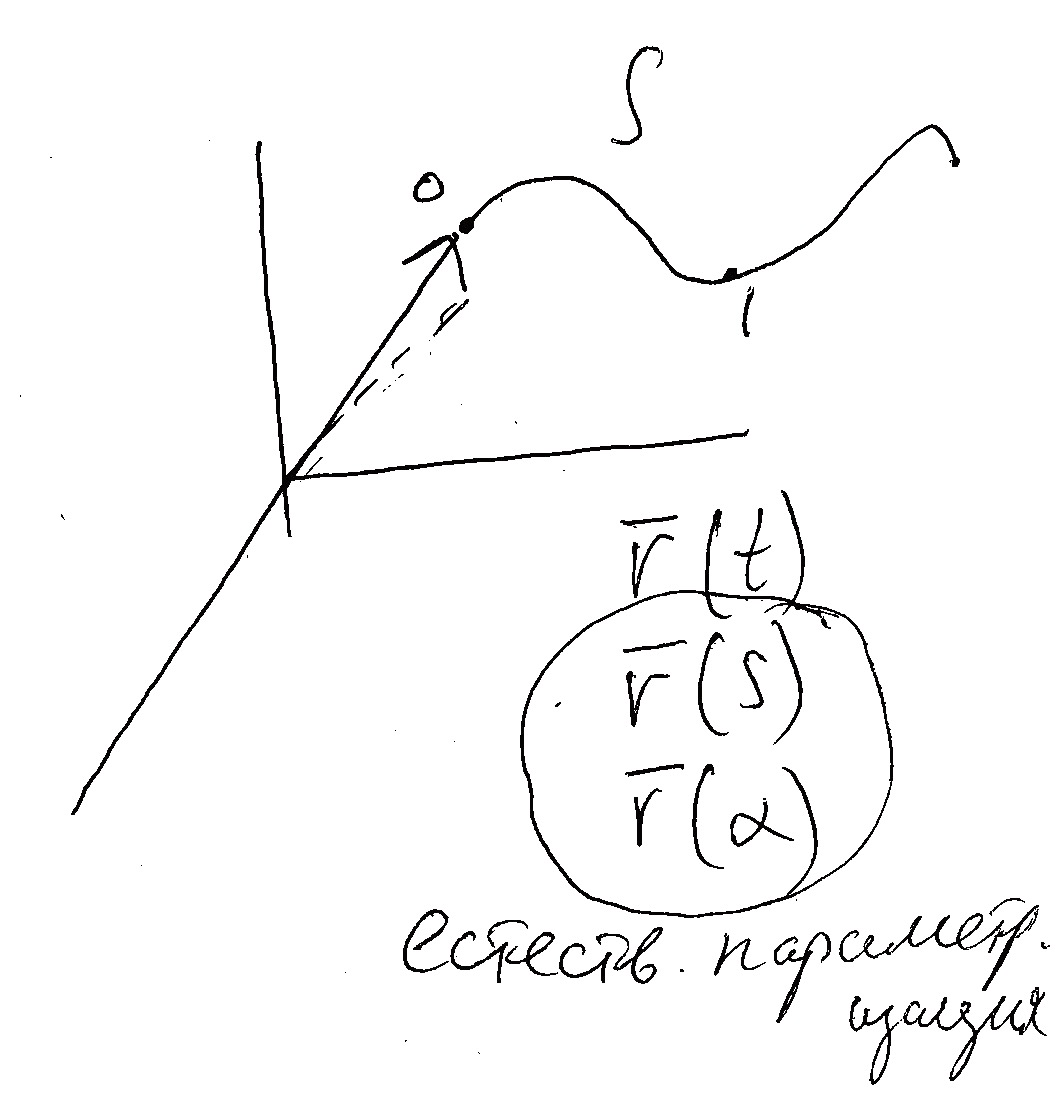
\includegraphics[width=0.5\textwidth]{ЕстественнаяПараметризация.jpg}
    \caption{}
    \label{fig:myimage} % Sets a label for cross-referencing
\end{figure}
\Def $\;$ Естественный способ задания движения:
\Def $\;$  Траектория геометрической точки - геометрическое место точек, занимаемых ей точек пространства  % FIXME не успел записать
\begin{enumerate}
    \item Траектория
    \item $S(t)$
\end{enumerate}
\paragraph{Длина траектории:}
\[S = \int_{\Gamma_{01}} dr\]
\[dr = \sqrt{\dot x^2 + \dot y^2 + \dot z^2} = \sqrt{v_x ^2 + v_y^2 + v_z^2} = v dt\]
\subsection*{Использование дифференциалов}
\begin{figure}[H]
    \centering
    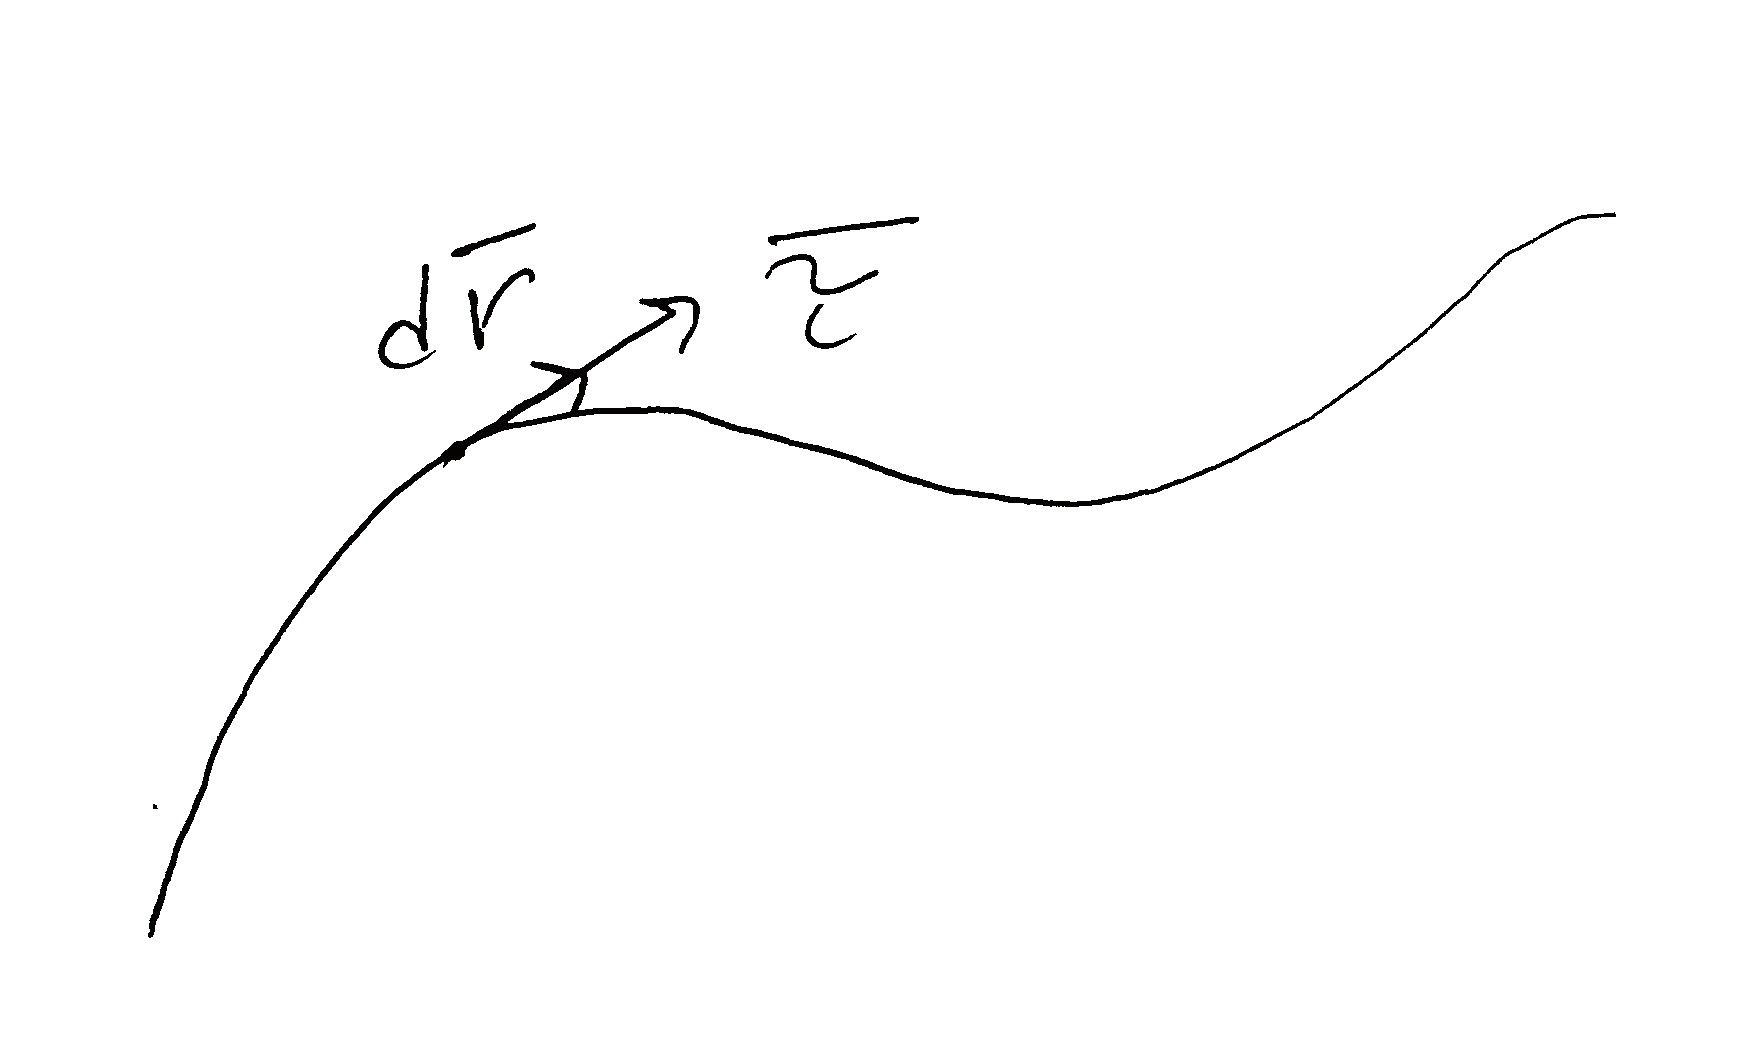
\includegraphics[width=0.5\textwidth]{КасательныйВектор.jpg}
    \caption{}
    \label{fig:myimage} % Sets a label for cross-referencing
\end{figure}
Касательный вектор $\bar \tau$:
\[\bar \tau = \frac{d \bar r}{ds} \; \; \; \; |\bar \tau| = 1\]
\[\bar v = \frac{d \bar r}{dt} = \frac{d \bar r}{d s} \cdot \frac{ds}{dt} = \bar \tau v \implies \bar \tau = \frac{\bar v}{v}\]

\subsection{Кривизна траектории}
\begin{figure}[H]
    \centering
    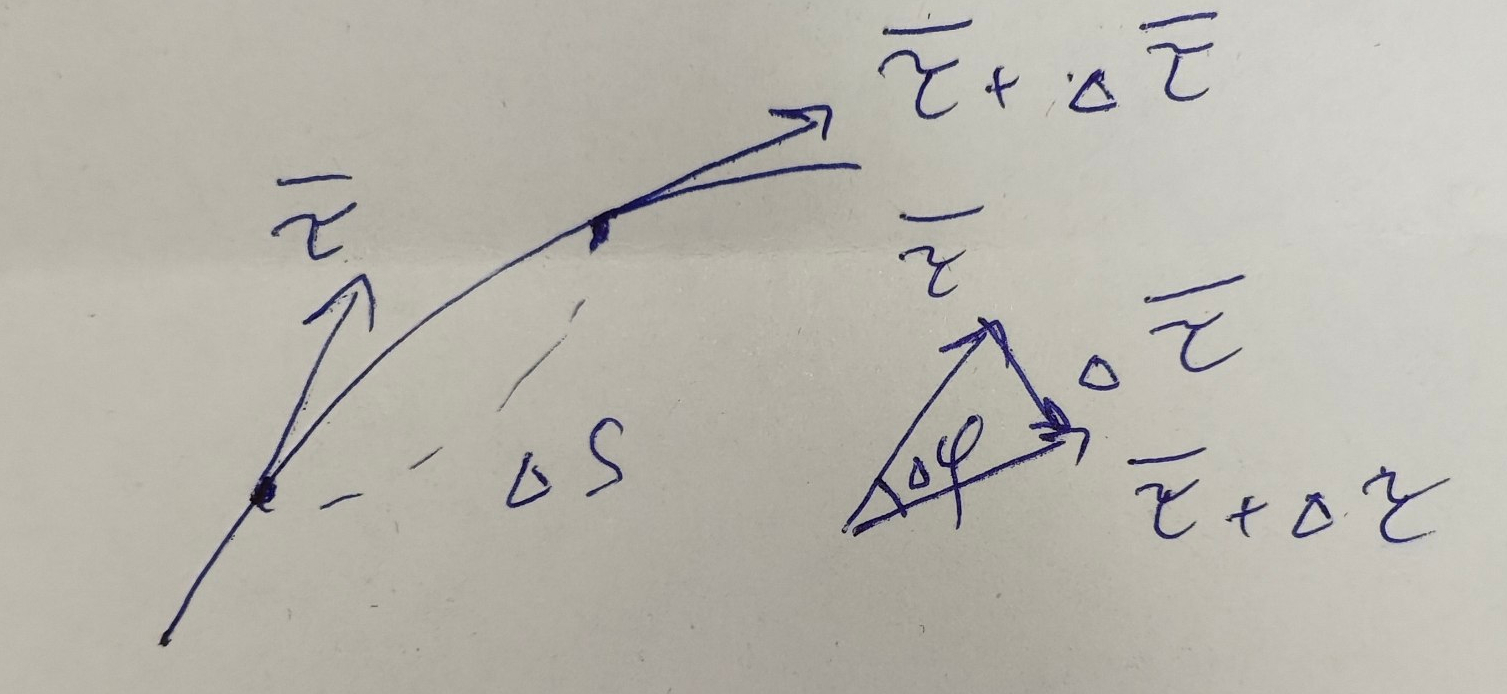
\includegraphics[width=0.5\textwidth]{Кривизна.jpg}
    \caption{}
    \label{fig:myimage} % Sets a label for cross-referencing
\end{figure}
\Def Кривизна
\[K := \lim_{\Delta s \to 0} \frac{\Delta \phi}{\Delta s} = \lim_{\Delta s \to 0} \frac{|\Delta \tau|}{|\bar \tau| \Delta s} = \left| \lim_{\Delta s \to 0} \frac{\Delta \bar \tau}{\Delta s} \right| = \left|\frac{d \bar \tau}{ds}\right|\]
\[1 = ( \bar \tau(s), \bar \tau(s)),\]
\[
0 = \left(\frac{d \bar \tau}{ds}, \bar \tau \right) + \left(\bar \tau , \frac{d \bar \tau}{ds}\right) = 2 \left(\frac{d \bar \tau}{ds}, \bar \tau\right) 
\]
\Def $\;$ Вектор главной нормали:
\[\bar n = \frac{d \bar \tau}{d s} / \left|\frac{d \tau}{ds}\right| = \frac{1}{K} \frac{d\bar \tau}{d s}\]
Из ранее доказанного:
\[(\bar n, \bar \tau) = 0\]
\Def $\;$ Вектор бинормали:
\[\bar b = \bar \tau \times \bar n\]
\[\bar w = \dot{\bar v} = \frac{d (\bar \tau, v)}{dt} = \frac{d \bar \tau}{dt} v + \bar \tau \frac{d \bar v}{dt} = \frac{d\bar \tau}{ds} \cdot \frac{ds }{dt} v  + \bar \tau \frac{d v}{dt} = \bar n k v^2 + \bar \tau \dot v\]
\Def \;
$k v^2 := w_n \; \; \; \;\dot v := w_\tau$ 
\\
\Def $\;$ Радиус кривизны
\[\rho := \frac{1}{K}\]
\[w_n= kv^2 = \frac{v^2}{\rho}\]

\paragraph{Касательные окружности соприкасаются,} когда разложение в ряд Тейлора совпадает до 2ой степени
\end{document}